\chapter{Graph Theory}
In this chapter we are going to discuss four problems from \blue{graph theory}.
\begin{enumerate}[(a)]
\item We present an algorithm to solve the 
      \href{https://en.wikipedia.org/wiki/Disjoint-set_data_structure}{\emph{union-find problem}}.
      In this problem, we are given a set $M$ and a relation $R \subseteq M \times M$.  Our task is
      then to find the \blue{equivalence relation} that is \blue{generated} by $R$.  The equivalence relation
      generated by the relation $R$ is the \blue{smallest equivalence relation} $\approx_R$ such that $R \subseteq\; \approx_R$.
      
      Essentially, the union-find problem is a mathematical problem.  Nevertheless, we will see that 
      it has an important practical application in computer science. 
\item The next problem we solve is the problem to compute the
      \href{https://en.wikipedia.org/wiki/Minimum_spanning_tree}{\emph{minimum spanning tree}}
      of a graph.  Given a weighted graph, this problem asks to find the smallest 
      \href{https://en.wikipedia.org/wiki/Glossary_of_graph_theory_terms#subgraph}{subgraph} that 
      connects all vertices of the graph.  We discuss
      \href{https://en.wikipedia.org/wiki/Kruskal%27s_algorithm}{Kruskal's algorithm} 
      for solving this problem.  
\item Then we discuss the problem of finding a shortest path in a 
      \href{https://en.wikipedia.org/wiki/Directed_graph}{\emph{weighted directed graph}}.
      We present \href{https://en.wikipedia.org/wiki/Dijkstra%27s_algorithm}{Dijkstra's algorithm} to solve
      this problem.   
\item Finally, we discuss \blue{topological sorting}.
\end{enumerate}

\section{The Union-Find Problem}
Assume that we are given a set $M$ together with a relation $R \subseteq M \times M$.  The relation
$R$ is not yet an  \href{https://en.wikipedia.org/wiki/Equivalence_relation}{equivalence relation} on $M$, but
this relation \blue{generates} an equivalence relation $\approx_R$ on $M$.  This
\blue{generated equivalence relation}\index{generated equivalence relation} is defined inductively. 
\begin{enumerate}
\item For every pair $\pair(x,y) \in R$ we have that $\pair(x, y) \in\; \approx_R$.

      This is the base case of the inductive definition.  It ensures that the relation
      $\approx_R$ is an \blue{extension} of the relation $R$, i.e.~it ensures that $R \subseteq\, \approx_R$.
\item For every $x \in M$ we have $\pair(x,x) \in\; \approx_R$.

      This ensures that the relation $\approx_R$ is \blue{reflexive}\index{reflexive} on $M$.
\item If $\pair(x,y) \in \approx_R$, then $\pair(y,x) \in\; \approx_R$.

      This  ensures that the relation $\approx_R$ is \blue{symmetric}.\index{symmetric}
\item If $\pair(x,y) \in\; \approx_R$ and $\pair(y,z) \in\; \approx_R$, then $\pair(x,z) \in\; \approx_R$.

      This clause ensures that the relation $\approx_R$ is \blue{transitive}.\index{transitive}
\end{enumerate}
Given this inductive definition, it can be shown that:
\begin{enumerate}[(a)]
\item $\approx_R$ is an equivalence relation on $M$.
\item If $Q$ is an equivalence relation on $M$ such that $R \subseteq Q$, then $\approx_R \subseteq Q$.
\end{enumerate}
Therefore, the relation $\approx_R$ is the \blue{smallest}
equivalence relation on $M$ that extends $R$.  In our lesson on
\href{https://github.com/karlstroetmann/Lineare-Algebra/blob/master/Skript/lineare-algebra.pdf}{Linear Algebra}
we had defined the transitive closure $R^+$ of a binary relation $R$ in a similar way.  In 
that lecture, we had then shown that $R^+$ is indeed the smallest transitive relation that extends
$R$.  This proof can easily be adapted to prove the claim given above.

It turns out that a direct implementation of the inductive definition of $\approx_R$ given above is
not very efficient.  Instead, we remind ourselves that there is are one-to-one correspondence
between the equivalence relations $R \subseteq M \times M$ and the
\href{https://en.wikipedia.org/wiki/Partition_of_a_set}{partitions} of $M$.  A set 
$\mathcal{P} \subseteq 2^M$ is a \blue{partition}\index{partition} of $M$ iff the following holds:
\begin{enumerate}
\item $\{\} \not\in \mathcal{P}$,
\item $A \in \mathcal{P} \wedge B \in \mathcal{P} \rightarrow A = B \vee A \cap B = \{\}$,
\item $\ds\bigcup \mathcal{P} = M$.
\end{enumerate}
Therefore, a partition $\mathcal{P}$ of $M$ is a subset of the power set of $M$ such that
every element of $M$ is a member of \magenta{exactly one} set of $\mathcal{P}$ and, furthermore, $\mathcal{P}$ must not contain the
empty set.  We have already seen in the lecture on Linear Algebra that an equivalence relation 
$\approx \;\subseteq M \times M$ gives rise to
\href{https://en.wikipedia.org/wiki/Equivalence_class}{equivalence classes}, 
where the \blue{equivalence class} generated by $x \in M$ is defined as
\\[0.2cm]
\hspace*{1.3cm}
$[x]_\approx := \{ y \mid \pair(x, y) \in\; \approx \}$.
\\[0.2cm]
It was then shown that the set of equivalence classes generated by all $x \in M$ 
\\[0.2cm]
\hspace*{1.3cm}
$\bigl\{ [x]_\approx \;\big|\; x \in M \bigr\}$
\\[0.2cm]
is a partition of $M$.  It was also shown that every partition $\mathcal{P}$ of a set $M$ gives rise
to an equivalence relation $\approx_\mathcal{P}$ that is defined as follows:
\\[0.2cm]
\hspace*{1.3cm}
$x \approx_\mathcal{P} y \;\Longleftrightarrow\; \exists A \in \mathcal{P}:(x \in A \wedge y \in A)$.
\\[0.2cm]
An example will clarify the idea.  Assume that
\\[0.2cm]
\hspace*{1.3cm}
$M := \{ 1,2,3,4,5,6,7,8,9 \}$.
\\[0.2cm]
Then the set 
\\[0.2cm]
\hspace*{1.3cm}
$\mathcal{P} := \bigl\{ \{ 1, 4, 7, 9\}, \{3, 5, 8\}, \{2, 6\} \bigr\}$
\\[0.2cm]
is a partition of $M$ since the three sets involved are disjoint and their union is the set $M$.
According to this partition, the elements $1$, $4$, $7$, and $9$ are all
equivalent to each other.  Similarly, the elements $3$, $5$, and $8$ are equivalent to each other,
and, finally, $2$ and $6$ are equivalent.

It turns out that, given a relation $R$, the most efficient way to compute the generated equivalence
relation $\approx_R$ is to compute the partition corresponding to this equivalence relation.  In
order to present the algorithm, we first sketch the underlying idea using a simple example.  Assume
the set $M$ is defined as
\\
\hspace*{1.3cm}
$M := \{ 1,2,3,4,5,6,7,8,9 \}$
\\[0.2cm]
and that the relation $R$ is given as follows:
\\[0.2cm]
\hspace*{1.3cm}
$R := \bigl\{ \pair(1,4), \pair(7,9), \pair(3,5), \pair(2,6), \pair(5,8), \pair(1,9), \pair(4,7) \bigr\}$.
\\[0.2cm]
Our goal is to compute a partition $\mathcal{P}$ of $M$ such that the formula
\\[0.2cm]
\hspace*{1.3cm}
$\pair(x, y) \in R \rightarrow \exists A \in \mathcal{P}:\bigl(x \in A \wedge y \in A)$
\\[0.2cm]
holds.  In order to achieve this goal, we define a sequence of partitions $\mathcal{P}_1$,
$\mathcal{P}_2$, $\cdots$, $\mathcal{P}_n$ such that $\mathcal{P}_n$ achieves our goal.
\begin{enumerate}
\item We start by defining
      \\[0.2cm]
      \hspace*{1.3cm}
      $\mathcal{P}_1 := \bigl\{ \{1\}, \{2\}, \{3\}, \{4\}, \{5\}, \{6\}, \{7\}, \{8\}, \{9\} \bigr\}$.
      \\[0.2cm]
      This is clearly a partition of $M$, but it is the trivial partition since it generates an equivalence
      relation $\approx$ where we have  $x \approx y$ if and only if $x = y$.  
\item Next, we have to ensure to incorporate our given relation $R$ into this partition.  Since $\pair(1,4) \in R$
      we replace the singleton sets $\{1\}$ and $\{4\}$ by their union.  This leads to the following
      definition of the partition $\mathcal{P}_2$:
      \\[0.2cm]
      \hspace*{1.3cm}
      $\mathcal{P}_2 := \bigl\{ \{1, 4\}, \{2\}, \{3\}, \{5\}, \{6\}, \{7\}, \{8\}, \{9\} \bigr\}$.
\item Since $\pair(7,9) \in R$, we replace the sets $\{7\}$ and $\{9\}$ by their union and define
      \\[0.2cm]
      \hspace*{1.3cm}
      $\mathcal{P}_3 := \bigl\{ \{1, 4\}, \{2\}, \{3\}, \{5\}, \{6\}, \{7, 9\}, \{8\} \bigr\}$.
\item Since $\pair(3,5) \in R$, we replace the sets $\{3\}$ and $\{5\}$ by their union and define
      \\[0.2cm]
      \hspace*{1.3cm}
      $\mathcal{P}_4 := \bigl\{ \{1, 4\}, \{2\}, \{3,5\}, \{6\}, \{7, 9\}, \{8\} \bigr\}$.
\item Since $\pair(2,6) \in R$, we replace the sets $\{2\}$ and $\{6\}$ by their union and define
      \\[0.2cm]
      \hspace*{1.3cm}
      $\mathcal{P}_5 := \bigl\{ \{1, 4\}, \{2,6\}, \{3,5\}, \{7, 9\}, \{8\} \bigr\}$.
\item Since $\pair(5,8) \in R$, we replace the sets $\{3,5\}$ and $\{8\}$ by their union and define
      \\[0.2cm]
      \hspace*{1.3cm}
      $\mathcal{P}_6 := \bigl\{ \{1, 4\}, \{2,6\}, \{3,5,8\}, \{7, 9\} \bigr\}$
\item Since $\pair(1,9) \in R$, we replace the sets $\{1,4\}$ and $\{7,9\}$ by their union and define
      \\[0.2cm]
      \hspace*{1.3cm}
      $\mathcal{P}_7 := \bigl\{ \{1, 4, 7, 9\}, \{2,6\}, \{3,5,8\} \bigr\}$
\item Next, we have $\pair(4,7) \in R$.  However, $4$ and $7$ are already in the same set.
      Therefore we do not have to change the partition $\mathcal{P}_7$ in this step.
      Furthermore, we have now processed all the pairs in the given relation $R$.
      Therefore, $\mathcal{P}_7$ is the partition that represents the equivalence relation $\approx$ generated
      by $R$.  According to this partition, we have found that
      \\[0.2cm]
      \hspace*{1.3cm}
      $1 \approx 4 \approx 7 \approx 9$, \quad $2 \approx 6$,  \quad and \quad $3 \approx 5 \approx 8$.
\end{enumerate}
 
\begin{figure}[!ht]
\centering
\begin{minted}[ frame         = lines, 
                framesep      = 0.3cm, 
                firstnumber   = 1,
                bgcolor       = sepia,
                numbers       = left,
                numbersep     = -0.2cm,
                xleftmargin   = 0.8cm,
                xrightmargin  = 0.8cm,
                ]{python3}
     def union_find(M, R):
        P = { frozenset({x}) for x in M } 
        for x, y in R:
            Sx = find(x, P)
            Sy = find(y, P)
            if Sx != Sy:
                P -= { Sx,  Sy }
                P |= { Sx | Sy }
        return P
    
    def arb(S):
        for x in S:
            return x
    
   def find(x, P):
        return arb({ S for S in P if x in S })    
\end{minted}
\vspace*{-0.3cm}
\caption{A naive implementation of the union-find algorithm.}
\label{fig:Union-Find-Naive.ipynb}
\end{figure}


What we have sketched in the previous example is known as the \blue{union-find algorithm}.\index{union-find algorithm}
Figure \ref{fig:Union-Find-Naive.ipynb} shows a naive implementation of this algorithm.  The
procedure $\mytt{unionFind}$ takes two arguments: $\mytt{M}$ is a set and $\mytt{R}$ is a relation
on $\mytt{M}$.  The purpose of $\mytt{unionFind}$ is to compute the equivalence relation $\approx_\mytt{R}$
that is generated by $\mytt{R}$ on $M$.  This equivalence relation is represented as a partition of $\mytt{M}$.
\begin{enumerate}
\item In line 2 we initialize $\mytt{P}$ as the trivial partition that contains only singleton
      sets.  Obviously, this is a partition of $\mytt{M}$ but it does not yet take the
      relation $\mytt{R}$ into account.
\item The \mytt{for}-loop in line 3 iterates over all pairs $(\mytt{x},\mytt{y})$ from $\mytt{R}$.
      First, we compute the set $\mytt{Sx}$ that contains $\mytt{x}$ and the set $\mytt{Sy}$ that
      contains $\mytt{y}$.  If these sets are not the same, then $\mytt{x}$ and $\mytt{y}$ are not
      yet equivalent with respect to the partition $\mytt{P}$.  Therefore, the equivalence classes
      $\mytt{Sx}$ and $\mytt{Sy}$ are joined and their union is added to the partition 
      $\mytt{P}$ in line 8, while the equivalence classes $\mytt{Sx}$ and $\mytt{Sy}$ are
      removed from $\mytt{P}$ in line 7.
\item The function \mytt{arb} takes a set $S$ as its argument and returns an
      arbitrary element from $S$. 
\item The function $\mytt{find}$ takes an element $\mytt{x}$ of a set $\mytt{M}$ and a partition
      $\mytt{P}$ of $\mytt{M}$.  Since $\mytt{P}$ is a partition of $\mytt{M}$ there must be exactly
      one set $\mytt{S}$ in $\mytt{P}$ such that $\mytt{x}$ is an element of $\mytt{S}$.  This set
      $\mytt{S}$ is then returned.
\end{enumerate}

\subsection{A Tree-Based Implementation}
The implementation shown in Figure \ref{fig:Union-Find-Naive.ipynb} is not very efficient.  The
problem is the computation of the union
\\
\hspace*{1.3cm}
$\mytt{Sx} \;|\; \mytt{Sy}$.
\\[0.2cm]
If the sets $\mytt{Sx}$ and $\mytt{Sy}$ are represented as ordered binary trees and, for the sake of the
argument, the set $\mytt{Sx}$ contains at most as many elements as the set $\mytt{Sy}$, then the
computational complexity of this operation is
\\
\hspace*{1.3cm}
$\Oh\bigl(\mytt{\#Sx} \cdot \log_2(\mytt{\#Sy})\bigr)$.  
\\[0.2cm]
The reason is that every element of $\mytt{Sx}$ has to be inserted into $\mytt{Sy}$ and this
insertion has a complexity of $\Oh\bigl(\log_2(\mytt{\#Sy})\bigr)$.  Here the expression
$\mytt{\#Sx}$ denotes the size of the set $\mytt{Sx}$ and similarly the expression
$\mytt{\#Sy}$ denotes the size of the set $\mytt{Sy}$.  A more efficient way to
represent these sets is via \blue{parent pointers}:  The idea is that every set is represented as a
tree.  However, this tree is not a binary tree but is rather represented by pointers that
point from a node to its parent.  The node at the root of the tree points to itself.  Then, taking the
union of two sets $\mytt{Sx}$ and $\mytt{Sy}$ is straightforward:  If $\mytt{rx}$ is the node at the root of
the tree representing $\mytt{Sx}$ and $\mytt{ry}$ is the node at the root of the tree representing
$\mytt{Sy}$, then changing the parent pointer of $\mytt{ry}$ to point to $\mytt{rx}$ merges the
sets \mytt{Sx} and \mytt{Sy}.


\begin{figure}[!ht]
\centering
\begin{minted}[ frame         = lines, 
                framesep      = 0.3cm, 
                firstnumber   = 1,
                bgcolor       = sepia,
                numbers       = left,
                numbersep     = -0.2cm,
                xleftmargin   = 0.0cm,
                xrightmargin  = 0.0cm,
              ]{python3}
    def find(x, Parent):
        if Parent[x] == x:
            return x
        return find(Parent[x], Parent)

    def union_find(M, R):
        Parent = { x: x for x in M } 
        for x, y in R:
            root_x = find(x, Parent)
            root_y = find(y, Parent)
            if root_x != root_y:
                Parent[root_y] = root_x
        Roots = { x for x in M if Parent[x] == x }
        return [{y for y in M if find(y, Parent) == r} for r in Roots]
\end{minted}
\vspace*{-0.3cm}
\caption{A tree-based implementation of the union-find algorithm.}
\label{fig:Union-Find-Tree.ipynb}
\end{figure}

Figure \ref{fig:Union-Find-Tree.ipynb} on page \pageref{fig:Union-Find-Tree.ipynb} shows an
implementation of this idea.  In this implementation, the parent pointers are represented using the
dictionary $\mytt{Parent}$.  
\begin{enumerate}
\item The function $\mytt{find}$ takes a node $\mytt{x}$ and the dictionary $\mytt{Parent}$ 
      that represents the parent pointers.  For a node $\mytt{y}$ the expression
      $\mytt{Parent}[\mytt{y}]$ returns the parent node of \mytt{y}.
      The purpose of the call $\mytt{find}(\mytt{x}, \mytt{Parent})$ is to
      return the root of the tree containing $\mytt{x}$.

      If $\mytt{x}$ is its own parent, then $\mytt{x}$ is already at the root of a tree and therefore 
      we can return $\mytt{x}$ itself in line 3.
      Otherwise, we compute the parent of $\mytt{x}$ and then recursively compute the root of the tree
      containing this parent.  
\item The function $\mytt{unionFind}$ takes a set $\mytt{M}$ and a relation $\mytt{R}$.  It returns
      a partition of $\mytt{M}$ that represents the equivalence relation generated by $\mytt{R}$ on
      $\mytt{M}$.  As I did not want to use \mytt{frozenset}s, this partition is represented by a list of
      sets. 

      The dictionary\footnote{
        In a language like \mytt{C} we would instead use pointers.  Of course, this would be more efficient.
      } $\mytt{Parent}$ is initialized in line 8 so that every node
      points to itself.   This corresponds to the fact that the sets in the initial partition are all
      singleton sets.  

      Next, the function $\mytt{unionFind}$ iterates over all pairs $\langle\mytt{x}, \mytt{y}\rangle$ from the binary
      relation $\mytt{R}$.  In line 9 and 10 we compute the roots of the trees containing $\mytt{x}$ and
      $\mytt{y}$.  If these roots are identical, then $\mytt{x}$ and $\mytt{y}$ are already
      equivalent and there is nothing to do.  However, if $\mytt{x}$ and $\mytt{y}$ are located 
      in different trees, then these trees need to be merged.  To this end, the parent pointer of
      the root of the tree containing $\mytt{y}$ is changed so that it 
      points to the root of the tree containing $\mytt{x}$.  Therefore, instead of iterating over all
      elements of the set containing $\mytt{y}$, we just change a single pointer.

      Line 13 computes the set of all nodes that are at the root of some tree.  Then, for every root
      $\mytt{R}$ of a tree, line 14 computes the set of nodes corresponding to this tree.
      These sets are collected in a list, which is then returned.
\end{enumerate}

\subsection{Controlling the Growth of the Trees}
As it stands, the algorithm shown in the previous section has a complexity that is $\Oh(n^2)$ in the
worst case where $n$ is the number of elements in the set $ \mytt{M}$.  The worst case happens if there
is just one equivalence class and the tree representing this class degenerates into a list.
Fortunately, it is easy to fix this problem if we keep track of the \blue{height} of the
different trees.  Then, if we want to join the trees rooted at $\mytt{parentX}$ and
$\mytt{parentY}$, we have a choice: We can either set the parent of the node $\mytt{parentX}$ to
be $\mytt{parentY}$ or we can set the parent of the node $\mytt{parentY}$ to be $\mytt{parentX}$.
If the tree rooted at $\mytt{parentX}$ is smaller than the tree rooted at $\mytt{parentY}$, then we should
attach this tree to the tree rooted at \mytt{parentY} via the assignment
\\[0.2cm]
\hspace*{1.3cm}
\mytt{parent[parentX] = parentY}
\\[0.2cm]
otherwise we should use the assignment
\\[0.2cm]
\hspace*{1.3cm}
\mytt{parent[parentY] = parentX}.
\\[0.2cm]
In order to be able to distinguish these cases, we store the height of the tree rooted at node
$\mytt{n}$ in the dictionary $\mytt{Height}$, i.e.~if $\mytt{n}$ is a node, then $\mytt{Height}[\mytt{n}]$ is
the height of the tree rooted at node $\mytt{n}$.  This yields the implementation shown in Figure
\ref{fig:Union-Find.ipynb} on page \pageref{fig:Union-Find.ipynb}.  Provided the size  of the relation
$\mytt{R}$ is bounded by the size $n$ of the set $ \mytt{M}$, the complexity of this
implementation is $\Oh\bigl(n \cdot \log(n)\bigr)$.  However, this excludes the last two lines of
the program.  In practice, the implementation of the function $\mytt{union\_find}$ would omit these
two lines and, instead, return the relation $\mytt{Parent}$ since this is all that is needed to
determine whether two elements $x$ and $y$ are equivalent. 

\begin{figure}[!ht]
\centering
\begin{minted}[ frame         = lines, 
                framesep      = 0.3cm, 
                firstnumber   = 1,
                bgcolor       = sepia,
                numbers       = left,
                numbersep     = -0.2cm,
                xleftmargin   = 0.0cm,
                xrightmargin  = 0.0cm,
              ]{python3}
    def union_find(M, R):
        Parent = { x: x for x in M } 
        Height = { x: 1 for x in M }
        for x, y in R:
            root_x = find(x, Parent)
            root_y = find(y, Parent)
            if root_x != root_y:
                if Height[root_x] < Height[root_y]:
                    Parent[root_x] = root_y
                elif Height[root_x] > Height[root_y]:
                    Parent[root_y] = root_x
                else:
                    Parent[root_y]  = root_x
                    Height[root_x] += 1
        Roots = { x for x in M if Parent[x] == x }
        return [{y for y in M if find(y, Parent) == r} for r in Roots]
\end{minted}
\vspace*{-0.3cm}
\caption{A more efficient version of the union-find algorithm.}
\label{fig:Union-Find.ipynb}
\end{figure}

\exercise
We can speed up the implementation previously shown if the set $\mytt{M}$ has the form
\\[0.2cm]
\hspace*{1.3cm}
$\mytt{M} = \{ 0, 1, 2, \cdots, n-1 \}$ \quad where $n \in \mathbb{N}$.
\\[0.2cm]
In this case, the relations $\mytt{Parent}$ and $\mytt{Height}$ can be implemented as arrays.
Develop an implementation that is based on this idea.
\eox

\exercise
For a natural number $h$, assume that $t_h$ is a tree of height $h$ that has been constructed with the union-find algorithm
discussed in this section and, furthermore, assume that this tree has the smallest number of nodes that is
possible for a tree of height $h$.  Define $c_h$ as the number of nodes in a tree $t_h$, set up an equation for
$c_h$ and solve this equation. \eox


\subsection{Packaging the  Union-Find Algorithm as a Class \label{sec:union-find-oo}}
Later, when we discus the problem of constructing a \blue{minimum spanning tree}, we will need the union-find algorithm as an
auxiliary data structure.  To this end we present a class that encapsulates the union-find
algorithm.  This class is shown in Figure \ref{fig:Union-Find-OO.ipynb} on page
\pageref{fig:Union-Find-OO.ipynb}.

\begin{figure}[!ht]
\centering
\begin{minted}[ frame         = lines, 
                framesep      = 0.3cm, 
                firstnumber   = 1,
                bgcolor       = sepia,
                numbers       = left,
                numbersep     = -0.2cm,
                xleftmargin   = 0.0cm,
                xrightmargin  = 0.0cm,
              ]{python3}
    class UnionFind:
        def __init__(self, M):
            self.mParent = { x: x for x in M }
            self.mHeight = { x: 1 for x in M }
            
        def find(self, x):
            p = self.mParent[x]
            if p == x:
                return x
            return self.find(p)

        def union(self, x, y):
            root_x = self.find(x)
            root_y = self.find(y)
            if root_x != root_y:
                if self.mHeight[root_x] < self.mHeight[root_y]:
                    self.mParent[root_x] = root_y
                elif self.mHeight[root_x] > self.mHeight[root_y]:
                    self.mParent[root_y] = root_x
                else:
                    self.mParent[root_y]  = root_x
                    self.mHeight[root_x] += 1
                    
    def partition(M, R):
        UF = UnionFind(M)
        for x, y in R:
            UF.union(x, y)
        Roots = { x for x in M if UF.find(x) == x }
        return [{y for y in M if UF.find(y) == r} for r in Roots]
\end{minted}
\vspace*{-0.3cm}
\caption{The class \mytt{unionFind}.}
\label{fig:Union-Find-OO.ipynb}
\end{figure}

\begin{enumerate}
\item The constructor $\mytt{unionFind}$ receives a set $\mytt{M}$ as arguments.  The class
      $\mytt{unionFind}$ maintains two variables:
      \begin{enumerate}
      \item $\mytt{mParent}$ is the dictionary implementing the pointers that point to the parents
             of each node.  If a node $\mytt{n}$ has no parent, then we have
             \\[0.2cm]
             \hspace*{1.3cm}
             \mytt{mParent[n] = n},
             \\[0.2cm]
             i.e.~the roots of the trees point to themselves.  Initially, all nodes are roots, so
             all parent pointers point to themselves.
      \item $\mytt{mHeight}$ is a dictionary containing the heights of the trees.  If $\mytt{n}$ is
            a node, then
            \\[0.2cm]
            \hspace*{1.3cm}
            \mytt{mHeight[n]}
            \\[0.2cm]
            gives the height of the subtree rooted at $\mytt{n}$. As initially all trees contain but
            a single node, these trees all have height $1$.
      \end{enumerate}
\item The method $\mytt{union}$ takes two nodes $\mytt{x}$ and $\mytt{y}$ and joins the trees that
      contain these nodes.  This is achieved by finding their parents $\mytt{parentX}$ and
      $\mytt{parentY}$.  Then, the root of the smaller of the two trees is redirected to point to
      the root of the bigger tree.
\item The method $\mytt{find}$ takes a node $\mytt{x}$ as its argument and computes the root of the
      tree containing $\mytt{x}$. 
\item The function $\mytt{partition}$ is a client of the class $\mytt{unionFind}$.  It takes a set
      $\mytt{M}$ and a relation $\mytt{R}$ on $\mytt{M}$ and computes a partition that corresponds
      to the equivalence relation generated by $\mytt{R}$ on $\mytt{M}$. 
      \begin{enumerate}
      \item First, the function constructs a union-find object $\mytt{UF}$ for the set $\mytt{M}$.
      \item Then the method iterates over all pairs $(\mytt{x},\mytt{y})$ in the relation $\mytt{R}$ and
            joins the equivalence classes corresponding to $\mytt{x}$ and $\mytt{y}$.
      \item Next, the method collects all nodes $\mytt{x}$ that are at the root of a tree.
      \item Finally, for every root $\mytt{R}$ the method collects those nodes $\mytt{x}$ that are
            part of the tree rooted at $\mytt{R}$.
      \end{enumerate}
      This method is only needed to test the implementation of the class \mytt{UnionFind}.
\end{enumerate}


\section{Minimum Spanning Trees}
Imagine a telecommunication company that intends to supply internet access to a developing country.
The capital of the country is located at the coast line and is already connected to the internet via
a submarine cable. It is the company's task to connect all of the towns and villages to the capital.
Since most parts of the country are covered by a dense jungle, it is cheapest to build the connecting lines
alongside existing roads.  However, it is not necessary to have connection lines at every road.  The task is to
compute the set of roads that have to be equipped with connection lines so that all cities are connected and
the overall cost of the connection is minimal.

Mathematically, this kind of problem can be formulated as the problem of
constructing a \href{https://en.wikipedia.org/wiki/Minimum_spanning_tree}{minimum spanning tree} for
a given \href{https://en.wikipedia.org/wiki/Graph_(discrete_mathematics)#Weighted_graph}{weighted}
\href{https://en.wikipedia.org/wiki/Graph_(discrete_mathematics)#Undirected_graph}{undirected graph}.
Next, we provide the definitions of those notions that are needed to formulate the minimum spanning
tree problem precisely.  Then, we present
\href{https://en.wikipedia.org/wiki/Kruskal%27s_algorithm}{Kruskal's algorithm} for solving the
minimum spanning tree problem. 

\subsection{Basic Definitions}
We start with the definition of an \blue{undirected graph}, which is a set of vertices that are connected by
undirected edges.  The formal definition follows.

\begin{Definition}[Undirected Graph]
  An \blue{undirected graph}\index{undirected graph} is a pair
   $\mathcal{G} = \langle \nodes, \edges\rangle$ such that
  \begin{enumerate}
  \item $\nodes$ is the set is a set of  \blue{nodes}.
  \item $\edges$ is the set of  \blue{edges}.\index{edge}  An edge $e$ has the form
        \\[0.2cm]
        \hspace*{1.3cm}
        $\{x, y\}$
        \\[0.2cm]
        and \blue{connects} $x$ and $y$.  Since $\{x,y\}$ is a set and therefore $\{x,y\} = \{y,x\}$, we have
        \\[0.2cm]
        \hspace*{1.3cm}
        $\{x,y\} \in \edges$ \quad if and only if \quad $\{y,x\} \in \edges$.
        \\[0.2cm]
        Hence, if $x$ is connected to $y$ then $y$ is also connected to $x$.

        We will further assume that if $\{x,y\}$ is an edge, then $x \not= y$, i.e.~we do not admit
        \href{https://en.wikipedia.org/wiki/Loop_(graph_theory)}{loops}. \index{loop}
  \end{enumerate}
\end{Definition}

Sometimes, the edges of an undirected graph have an associated weight.  This leads to the notion of a
\blue{weighted undirected graph} that is given next.

\begin{Definition}[Weighted Graph] A \blue{weighted undirected graph}\index{weighted undirected graph} is a triple 
   $\langle \nodes, \edges, \weight{\cdot} \rangle$ such that
  \begin{enumerate}
  \item $\langle \nodes, \edges \rangle$ is an undirected graph.
  \item $\weight{\cdot}: \edges \rightarrow \N$ is a function assigning a \blue{weight}\index{weight of an edge} to every edge.

        In practical applications, the weight of an edge is often interpreted as the \blue{cost} or the
        \blue{length} of the edge.
        \eoxs
  \end{enumerate}
\end{Definition}

\noindent
Given an undirected graph $\mathcal{G} = \langle \nodes, \edges \rangle$, a \blue{path}\index{path} $P$
in $\mathcal{G}$ is a list of the form 
\\[0.2cm]
\hspace*{1.3cm} 
$P = [ x_0, x_1, x_2, \cdots, x_n ]$ 
\\[0.2cm]
such that we have : \\[0.2cm]
\hspace*{1.3cm}
$\{x_i,x_{i+1}\} \in \edges$  \quad for all $i = 0, \cdots, n-1$.
\\[0.2cm]
The set of all paths is denoted as $\mathbb{P}$, i.e.~we define
\\[0.2cm]
\hspace*{1.3cm}
$\ds \mathbb{P}  := \bigl\{ P \mid \mbox{$P$ is a path} \bigr\}$.
\\[0.2cm]
A path $P = [ x_0, x_1, \cdots, x_n]$ \blue{connects} the nodes $x_0$ and $x_n$.  The \blue{weight} of a
path\index{weight of an path} is defined as
the sum of the weights of all of its edges.  
\\[0.2cm]
\hspace*{1.3cm}
 $\ds\Weight{[x_0,x_1, \cdots, x_n]} \df \sum\limits_{i=0}^{n-1} \Weight{\{x_i,x_{i+1}\}}$. 
\\[0.2cm]
A graph is \blue{connected}\index{connected graph}\index{connected graph} if for every $x,y \in \nodes$ there is a path connecting $x$ and $y$, i.e.~we have
\\[0.2cm]
\hspace*{1.3cm}
$\forall x, y \in \mathbb{V}: \exists P \in \mathbb{P}: \bigl(P[0] = x \wedge P[\mytt{len}(P)-1] = y\bigr)$.
\\[0.2cm]
A set of edges can be interpreted as graph since the set of nodes can be computed from the edges as
follows: 
\\[0.2cm]
\hspace*{1.3cm}
$\ds\nodes = \bigcup \bigl\{\{x,y\} \,\big|\, \{x,y\} \in \edges \bigr\}$.
\\[0.2cm]
Then, a set of edges $\edges$ is called a \blue{tree}\index{tree (graph)} if and only if
\begin{enumerate}[(a)]
\item the corresponding graph is connected \quad \textbf{and}
\item removing any edge from $\edges$ would result in a graph that is no longer connected.
\end{enumerate}
These conditions can be restated: A tree is a connected graph that does not have a \blue{cycle}.
Here, a \blue{cycle} is a path of the form $[x_0, x_1, \cdots, x_n]$ where $n > 0$ and $x_0 = x_n$.  

\begin{Definition}[Weight of a Tree]
We define the \blue{weight} of a tree \index{weight of a tree} as the sum of the weights of its edges,
i.e.~if the Graph $\mathcal{G} = (\mathbb{V},\mathbb{E}, \weight{\cdot})$ is a tree, then
\\[0.2cm]
\hspace*{1.3cm}
$\ds \mytt{weight}(\mathcal{G}) := \sum\limits_{\{x,y\} \in \mathbb{E}} \Weight{\{x,y\}}$.  \eoxs
\end{Definition}

\begin{Proposition}
  Assume that $\mathcal{T} = (\mathbb{V},\mathbb{E})$ is an undirected graph that does not contain a
  cycle.  Then $\mathcal{T}$ is a tree if and only if $\#\mathbb{E} = \#\mathbb{V} - 1$ holds.  Here, $\#\mathbb{E}$ denotes the number of edges,
  while $\#\mathbb{V}$ denotes the number of vertices.  
\end{Proposition}

\proof
We will show the following claims:
\begin{enumerate}[(a)]
\item If the number of edges $\# \mathbb{E}$ is greater than $\#\mathbb{V}-1$, then $\mathcal{T}$ has to contain a cycle.
\item If the number of edges $\# \mathbb{E}$ is smaller than  $\#\mathbb{V}-1$, then $\mathcal{T}$ cannot be connected.
\item If the number of edges $\# \mathbb{E}$ is equal to $\#V - 1$, then $\mathcal{T}$ is a tree.
\end{enumerate}
We prove all of these claims simultaneously by induction on $n := \#V$.
\begin{enumerate}
\item[B.C.:] $n = 1$.

  If the graph contains only 1 vertex, we have $\mathbb{V} = \{x\}$ and hence the set of edges $\mathbb{E}$
  must be empty. Therefore we have
  \\[0.2cm]
  \hspace*{1.3cm}
  $\#\mathbb{V} = 1$, \quad $\#\mathbb{E} = 0$, \quad and therefore \quad $\#\mathbb{E} = \#\mathbb{V}-1$.
  \\[0.2cm]
  Hence the first two claims are vacuously true because their precondition is never satisfied.
  Furthermore, in that case the graph trivially is a tree and thus the third claim is true.
\item[I.S.:] $1, 2, \cdots, n-1 \mapsto n$

  In this case we pick any edge $\{x,y\}$ from $\mathbb{E}$ and define a new graph $\mathcal{T}'$ that results from $\mathcal{T}$
  by removing the edge $\{x,y\}$ from $\mathbb{E}$:
  \\[0.2cm]
  \hspace*{1.3cm}
  $\mathcal{T}' := \bigl\langle \mathbb{V}, \mathbb{E} \backslash \bigl\{ \{x,y\} \bigr\} \bigr\rangle$ 
  \\[0.2cm]
  Next, we define $A$ to be the set of those vertices that are connected to $x$ in $\mathcal{T}'$, $B$ to be the set
  of vertices that are connected to $y$ in $\mathcal{T}'$, and $C$ to contain those vertices that are neither connected to
  $x$ nor to $y$:
  \begin{enumerate}[(a)]
  \item $A := \{ z \in \mathbb{V} \mid \mbox{$z$ is connected to $x$ in $\mathcal{T}'$}\}$, \quad 
  \item $B := \{ z \in \mathbb{V} \mid \mbox{$z$ is connected to $y$ in $\mathcal{T}'$}\}$, \quad and \quad
  \item $C := \{ z \in \mathbb{V} \mid \mbox{$z$ is neither connected to neither $x$ nor to $y$}\}$.
  \end{enumerate}
  The sets $A$ and $B$ have to be disjoint, for if there were a vertex $z$ such that $z$ were connected to both
  $x$ and $y$, then the graph $T$ would contain a cycle.  If $\{u,v\}\in\mathbb{E}$, then there are three cases:
  \begin{enumerate}[(a)]
  \item $u$ is connected to $x$.  Because $\{u,v\}\in\mathbb{E}$ this implies that then $v$ is also connected
        to $x$ and hence both $u$ and $v$ are in $A$.
  \item $u$ is connected to $y$.  Then $v$ is also connected to $y$ and hence $u$ and $v$ are in $B$.
  \item $u$ is neither connected to $x$ nor to $y$.  Then $v$ can't be connected to $x$ or $y$ either.
        Therefore, both $u$ and $v$ are in the set $C$.
  \end{enumerate}
  Accordingly, we can split the set $\mathbb{E}$ of edges into three disjoint parts:
  \begin{enumerate}[(a)]
  \item $\mathbb{E}_A := \bigl\{ \{u,v\}\in\mathbb{E} \mid u\in A \wedge v\in A \bigr\}$,
  \item $\mathbb{E}_B := \bigl\{ \{u,v\}\in\mathbb{E} \mid u\in B \wedge v\in B \bigr\}$,
  \item $\mathbb{E}_C := \bigl\{ \{u,v\}\in\mathbb{E} \mid u\not\in A \cup B \wedge v\not\in A \cup B \bigr\}$.
  \end{enumerate}
  Then, we can define three graphs $\mathcal{T}_A$, $\mathcal{T}_B$, and $\mathcal{T}_C$ as follows:
  \begin{enumerate}[(a)]
  \item $\mathcal{T}_A = \langle A, \mathbb{E}_A \rangle$,
  \item $\mathcal{T}_B = \langle B, \mathbb{E}_B \rangle$,
  \item $\mathcal{T}_C = \langle C, \mathbb{E}_C \rangle$,
  \end{enumerate}
  As the graph $\mathcal{T}$ does not contain a cycle, the graphs $\mathcal{T}_A$, $\mathcal{T}_B$, and $\mathcal{T}_C$ can't contain a cycle either,
  since they are subgraphs of $\mathcal{T}$.  Next, we define $a := \# A$, $b := \# B$, and $c := \# C$.
  Since $a < n$, $b < n$, and $c < n$ by induction hypothesis the claim holds true for  $\mathcal{T}_A$, $\mathcal{T}_B$, and
  $\mathcal{T}_C$.  Let us assume that $\# \mathbb{E}_A > a - 1$.  By induction hypothesis we could then conclude that
  $\mathcal{T}_A$ contains a cycle.  This would imply that also $\mathcal{T}$ contains a cycle and since this would contradict our
  assumption, we can conclude that
  \\[0.2cm]
  \hspace*{1.3cm}
  $\# \mathbb{E}_A \leq a - 1$.
  \\[0.2cm]
  In a similar way we must also have
  \\[0.2cm]
  \hspace*{1.3cm}
  $\# \mathbb{E}_B \leq b - 1$ \quad and \quad $\# \mathbb{E}_C \leq c - 1$.
  \\[0.2cm]
  Now there are three cases.
  \begin{enumerate}
  \item Case: $C = \emptyset$, $\mathbb{E}_A = a - 1$, and $\mathbb{E}_B = b - 1$.
    
    Then by induction hypothesis $\mathcal{T}_A$ and $\mathcal{T}_B$ are trees.  In that case, $\mathcal{T}$ is
    a tree also because the edge $\{x,y\}$ connects the nodes from $A$ and $B$.
    Since $\mathbb{E} = \mathbb{E}_A + \mathbb{E}_B + 1$ and $n = a + b$ we have
    \\[0.2cm]
    \hspace*{1.3cm}
    $\mathbb{E} = (a - 1) + (b - 1) + 1 = n - 1 = \#\mathbb{V} - 1$.
    \\[0.2cm]
    Hence in this case the claims $(a)$ and $(b)$  are trivially true as their assumptions are not given,
    while the last claim is true because $\mathcal{T}$ is a tree.
    \green{$\surd$}
  \item Case: $C = \emptyset$, $\mathbb{E}_A < a - 1$, or $\mathbb{E}_B < b - 1$.
    
    Then by induction hypothesis either $\mathcal{T}_A$ or $\mathcal{T}_B$ is not connected.  Of course, then $\mathcal{T}$ is not connected either.
    Furthermore, since we have $\# \mathbb{E}_A \leq a - 1$ and $\# \mathbb{E}_B \leq b - 1$ it follows that
    \\[0.2cm]
    \hspace*{1.3cm}
    $\mathbb{E} = \mathcal{E}_A + \mathbb{E}_B - 1 < (a - 1) + (b - 1) = n - 1 = \#\mathbb{V} - 1$.
    \\[0.2cm]
    Therefore in this case claim $(a)$ and $(c)$ are trivially true and $(b)$ is true because $\mathcal{T}$ is
    not connected.  \green{$\surd$}
  \item Case $C \not= \emptyset$.

    In that case the graph $\mathcal{T}$ can't be connected since the vertices in $C$ are not connected to either $x$ or
    $y$.  Furthermore, we have
    \\[0.2cm]
    \hspace*{1.3cm}
    $\# \mathbb{E}_A + \# \mathbb{E}_B + \# \mathbb{E}_C \leq a + b + c - 3$.
    \\[0.2cm]
    Since we have
    \\[0.2cm]
    \hspace*{1.3cm}
    $\mathbb{E} = \mathbb{E}_A \uplus \mathbb{E}_B \uplus \mathbb{E}_C \uplus \bigl\{\{x,y\}\bigr\}$
    \\[0.2cm]
    and, furthermore, $n = a + b + c$, we know that
    \\[0.2cm]
    \hspace*{1.3cm}
    $\#\mathbb{E} = \#\mathbb{E}_A + \#\mathbb{E}_B + \#\mathbb{E}_C + 1$.
    \\[0.2cm]
    Therefore it follows that $\mathbb{E} \leq n - 2 < n - 1 = \#\mathbb{V} - 1$.
    \\[0.2cm]
    Therefore in this case claim $(a)$ and $(c)$ are trivially true and $(b)$ is true because $\mathcal{T}$ is
    not connected.  \green{$\surd$}
  \end{enumerate}
  Hence the claim has been established in all three cases. \qed
\end{enumerate} 

\subsection{Kruskal's Algorithm}
In 1956 the mathematician \href{https://en.wikipedia.org/wiki/Joseph_Kruskal}{Joseph Bernard Kruskal} (1928 -- 2010) 
found a very elegant algorithm for solving the minimum spanning tree problem.   This algorithm makes use
of the \blue{union-find algorithm} that we have shown in the previous section.  The basic idea is as
follows.\index{Kruskal's algorithm}
\begin{enumerate}[(a)]
\item In the first step, we create a union-find data structure that contains \blue{singleton trees}
      for all nodes in the graph.  Here, a singleton tree is a tree containing just a single node.
\item Next, we iterate over all edges $\pair(x, y)$ in the graph in \blue{increasing order of their weight}.
      If the nodes $x$ and $y$ are not yet connected, we join their respective equivalence classes by adding
      the edge $\pair(x, y)$ to the tree we are building.

      The fact that we investigate the edges in increasing order of their weight implies that we always choose
      the \blue{cheapest} edge to connect two nodes that are not yet connected.  Hence, Kruskal's algorithm is
      known as a \href{https://en.wikipedia.org/wiki/Greedy_algorithm}{greedy algorithm}.
\item We stop when the number of edges is one less than the number of nodes since, according to the
      proposition in the previous section, the tree must then connect all the nodes of the graph. 
\end{enumerate}
The fact that we iterate over the edges in increasing order of their weight guarantees that the
resulting tree has a minimal weight.
The algorithm is shown in Figure \ref{fig:Kruskal.ipynb} on page \pageref{fig:Kruskal.ipynb}.  We
discuss this program next.

\begin{figure}[!ht]
\centering
\begin{minted}[ frame         = lines, 
                framesep      = 0.3cm, 
                firstnumber   = 1,
                bgcolor       = sepia,
                numbers       = left,
                numbersep     = -0.2cm,
                xleftmargin   = 0.8cm,
                xrightmargin  = 0.8cm,
              ]{python3}
    import heapq         as hq

    def mst(V, E):
        UF  = UnionFind(V)
        MST = set()         # minimum spaning tree
        H   = []            # empty priority queue for edges
        for edge in E:
            hq.heappush(H, edge)
        while True:
            w, (x, y) = hq.heappop(H)
            root_x = UF.find(x)
            root_y = UF.find(y)
            if root_x != root_y:
                MST.add((w, (x, y)))
                UF.union(x, y)
                if len(MST) == len(V) - 1:
                    return MST
\end{minted}
\vspace*{-0.3cm}
\caption{Kruskal's algorithm.}
\label{fig:Kruskal.ipynb}
\end{figure}

\begin{enumerate}
\item Initially, we import the module \mytt{union\_find\_oo}, which is the object oriented 
      implementation of the union-find algorithm that has been presented in Section \ref{sec:union-find-oo}.
\item Furthermore, we import the module \mytt{heapq} as it provides us with a priority queue.
\item The main function is the function $\mytt{mst}$, which is short for \underline{m}inimum
      \underline{s}panning \underline{t}ree.  This function takes two arguments:
      $\mytt{V}$ is the set of nodes and $\mytt{E}$ is the set of edges of a given graph.  The edges are represented as
      pairs of the form
      \\[0.2cm]
      \hspace*{1.3cm}
      $\bigl(\mytt{w}, (\mytt{x}, \mytt{y})\bigr)$.
      \\[0.2cm] 
      Here, $\mytt{x}$ and $\mytt{y}$ are the nodes connected by the edge and $\mytt{w}$ is the
      weight of the edge.  The function $\mytt{mst}$ computes a minimum spanning tree of  the
      graph  $\pair(\mytt{V},\mytt{E})$.  It is assumed that this graph is connected.
\item The function $\mytt{mst}$ first creates the union-find data structure $\mytt{UF}$ in line 5.
      Initially, every node in $\mytt{UF}$ is  an equivalence class all by itself, i.e.~no nodes
      are connected.
\item The spanning tree constructed by the algorithm is stored in the variable $\mytt{MST}$.
      The spanning tree is represented by the set of its weighted edges.  
\item Next, the set of weighted edges $\mytt{E}$ is turned into a priority queue.
      We use the weights of the edges as priorities. 
      To this end, we create an empty priority queue $\mytt{H}$ in line 7.
      The \mytt{for}-loop in line 8-9 inserts all edges of the set \mytt{E} into this priority queue.
\item The \mytt{while}-loop in line 10 checks for every edge $(\mytt{x},\mytt{y})$  whether $\mytt{x}$ and $\mytt{y}$ are already
      connected.  This is the case if both $\mytt{x}$ and $\mytt{y}$ are part of the same tree
      in the union-find data structure \mytt{UF}.  In order to
      check whether $\mytt{x}$ and $\mytt{y}$ are part of the same tree
      we have to compute the roots of these trees. 
      If these roots are identical, then \mytt{x} and \mytt{y} are part of the same tree and hence
      they are already connected. 
\item If $\mytt{x}$ and $\mytt{y}$ are not yet connected, the  edge $(\mytt{w}, (\mytt{x}, \mytt{y}))$ is added to the
      spanning tree and the trees containing $\mytt{x}$ and $\mytt{y}$ are connected by calling the function
      \mytt{union}.
\item The algorithm terminates once the tree \mytt{MST} has $\mytt{\#V-1}$ edges, since we know from the previous
      exercise that in this case all nodes are connected by the edges in \mytt{MST}.
\end{enumerate}


\section{Shortest Paths Algorithms}
In this section we will show two algorithms that solve the
\href{https://en.wikipedia.org/wiki/Shortest_path_problem}{\blue{shortest path problem}}, the 
\href{https://en.wikipedia.org/wiki/Bellman-Ford_algorithm}{Bellman-Ford algorithm} and
\href{https://en.wikipedia.org/wiki/Dijkstra%27s_algorithm}{Dijkstra's algorithm}.  
In order to explain the shortest path problem and the algorithms to solve it, we introduce the notion
of a \href{https://en.wikipedia.org/wiki/Directed_graph}{\blue{weighted directed graph}}.


\begin{Definition}[Weighted Digraph] \
  A \blue{weighted directed graph}\index{weighted directed graph}
  (a.k.a.~a \blue{weighted digraph}\index{weighted digraph}) is a triple $\langle \nodes, \edges, \weight{\cdot} \rangle$ such that
  \begin{enumerate}
  \item $\nodes$ is the set of \blue{nodes} (sometimes the nodes are known as \blue{vertices}).
  \item $\edges \subseteq \nodes \times \nodes$ is the set of \blue{edges}.
  \item $\weight{\cdot}: \edges \rightarrow \N$ is a function that assigns a positive \blue{length} 
        to every edge.  This length is also known as the \blue{weight} of the edge.
        \eoxs
  \end{enumerate}
\end{Definition}

\remark
The main difference between a \blue{graph} and a \blue{digraph} is that in a digraph the edges are 
\mbox{p\hspace{-0.15cm}\underline{\hspace{0.15cm}airs}} of two
nodes while in a graph the edges are \underline{sets} of two nodes.  Informally, the edges in a
digraph can be viewed as one-way streets, while in a graph they represent streets that can be used in both
directions.  Hence, if a digraph has an edge $\pair(a,b)$, then this edge enables us to get from $a$ to $b$ but
this edge does not enable us to go from $b$ to $a$.  On the other hand, if a graph has an edge $\{a,b\}$, then
this edge enables us to go from $a$ to $b$ as well as to go from $b$ to $a$.
\eoxs

\begin{Definition}[Path, Path Length]
 A \blue{path} $P$ in a digraph \index{path} is a list of the form 
\\[0.2cm]
\hspace*{1.3cm} 
$P = [ x_0, x_1, x_2, \cdots, x_n ]$ 
\\[0.2cm]
such that
\\[0.2cm]
\hspace*{1.3cm} $\pair(x_i,x_{i+1}) \in \edges$ \quad holds for all $i = 0, 1, \cdots, n-1$. 
\\[0.2cm]
The set of all paths is denoted as $\paths$.
The length of a path is the sum of the length of all edges:
\\[0.2cm]
\hspace*{1.3cm}
$\ds\Weight{[x_0,x_1, \cdots, x_n]} \df \sum\limits_{i=0}^{n-1} \Weight{\pair(x_i,x_{i+1})}$. 
\\[0.2cm]
If  $p = [x_1, x_2, \cdots, x_n]$ is a path then  $p$ \blue{connects} \index{connect, path} the node $x_1$ with the node
$x_n$.  We denote the set of all paths that connect the node $v$ with the node $w$ as
\index{$\paths(v,w)$}
\\[0.2cm]
\hspace*{1.3cm} 
 $\paths(v,w) \df \bigl\{ [x_0, x_1, \cdots, x_n] \in \paths \bigm| x_0 = v \,\wedge\, x_n = w \bigr\}$.
\end{Definition}

\noindent
Now we are ready to state the shortest path problem.

\begin{Definition}[Shortest Path Problem] \lb
  Assume a weighted digraph  
  $G = \langle \nodes, \edges, \weight{\cdot} \rangle$ 
  and a node $\source \in \nodes$ is given.  Then the \blue{shortest path problem} \index{shortest path problem}
  asks to compute the following function:
  \\[0.2cm]
  \hspace*{1.3cm} $\spath: \nodes \rightarrow \N$ \\[0.1cm]
  \hspace*{1.3cm} $\spath(v) \df \mytt{min}\bigl\{ \weight{p} \bigm| p \in \paths(\source,v) \bigr\}$.
  \\[0.2cm]
  \index{$\spath(v)$}
  Furthermore, given that $\spath(v) = n$, we would like to be able to compute a path 
  $p \in \paths(\source,v)$ such that $\weight{p} = n$.
  \eox
\end{Definition}

\subsection{The Bellman-Ford Algorithm}
The first algorithm we discuss is the
\href{https://en.wikipedia.org/wiki/Bellman-Ford_algorithm}{Bellman-Ford algorithm}.
\index{Bellman-Ford algorithm}
It is named after the mathematicians 
\href{https://en.wikipedia.org/wiki/Richard_E._Bellman}{Richard E.~Bellman} \cite{bellman:58} and 
\href{https://en.wikipedia.org/wiki/L._R._Ford_Jr.}{Lester R.~Ford Jr.} \cite{ford:56} who discovered this algorithm
independently and published their results in 1958 and 1956, respectively.  Figure
\ref{fig:Moore.ipynb} on page \pageref{fig:Moore.ipynb} shows the implementation of a variant of this 
algorithm in \textsl{Python}.  This variant of the algorithm was suggested by 
\href{https://en.wikipedia.org/wiki/Edward_F._Moore}{Edward F.~Moore} \cite{moore:59} \index{Moore's algorithm}
in 1959.


\begin{figure}[!ht]
  \centering
\begin{minted}[ frame         = lines, 
                framesep      = 0.3cm, 
                firstnumber   = 1,
                bgcolor       = sepia,
                numbers       = left,
                numbersep     = -0.2cm,
                xleftmargin   = 0.8cm,
                xrightmargin  = 0.8cm,
              ]{python3}
    def shortest_path(source, Edges):
        Distance = { source: 0 }
        Fringe   = [ source ]
        while len(Fringe) > 0:
            u = Fringe.pop()
            for v, l in Edges[u]:
                dv = Distance.get(v, None)
                if dv == None or Distance[u] + l < dv:
                    Distance[v] = Distance[u] + l
                    if v not in Fringe: 
                        Fringe = Fringe + [v] 
        return Distance
\end{minted}
\vspace*{-0.3cm}
  \caption{The Bellman-Ford algorithm to solve the shortest path problem.}
  \label{fig:Moore.ipynb}
\end{figure} 

\noindent
\begin{enumerate}
\item The function $\mytt{shortestPath}(\mytt{source}, \mytt{Edges})$ is called with two arguments:
      \begin{enumerate}
      \item $\mytt{source}$ is the start node.  The task of the function
            $\mytt{shortestPath}(\mytt{source}, \mytt{Edges})$ is to compute the distances of all 
            vertices from the node $\mytt{source}$.
      \item $\mytt{Edges}$ is a \blue{dictionary} that encodes the set of edges of the graph.  For
            every node $x$ the value of $\mytt{Edges}[x]$ has the form
            \\[0.2cm]
            \hspace*{1.3cm}
            $\bigl[ (y_1, l_1), \cdots, (y_n, l_n) \bigr]$.
            \\[0.2cm]
            This list is interpreted as follows: For every $i = 1,\cdots,n$ there is an edge
            $(x, y_i)$ pointing from $x$ to $y_i$ and this edge has the length $l_i$.

            For example, the dictionary $\mytt{Edges}$ given below defines a simple digraph.
            In that digraph, there is an edge from node $\mytt{"a"}$ to node $\mytt{"c"}$ which has a
            length of $2$ and there is another edge from node $\mytt{"a"}$ to the node $\mytt{"b"}$ that has a length of $9$.
            \begin{verbatim}
    Edges = { 'a': [('c', 2), ('b', 9)], 
              'b': [('d', 1)],
              'c': [('e', 5), ('g', 3)],  
              'd': [('f', 2), ('e', 4)],  
              'e': [('f', 1), ('b', 2)],
              'f': [('h', 5)],
              'g': [('e', 1)],
              'h': []
            }
            \end{verbatim}
      
      The directed graph defined by this dictionary is shown in Figure \ref{fig:directed-graph.pdf}.
      In this Figure, every node is labelled both with its name and its distance from the source node \mytt{a}.
      \begin{figure}[!ht]
        \centering
        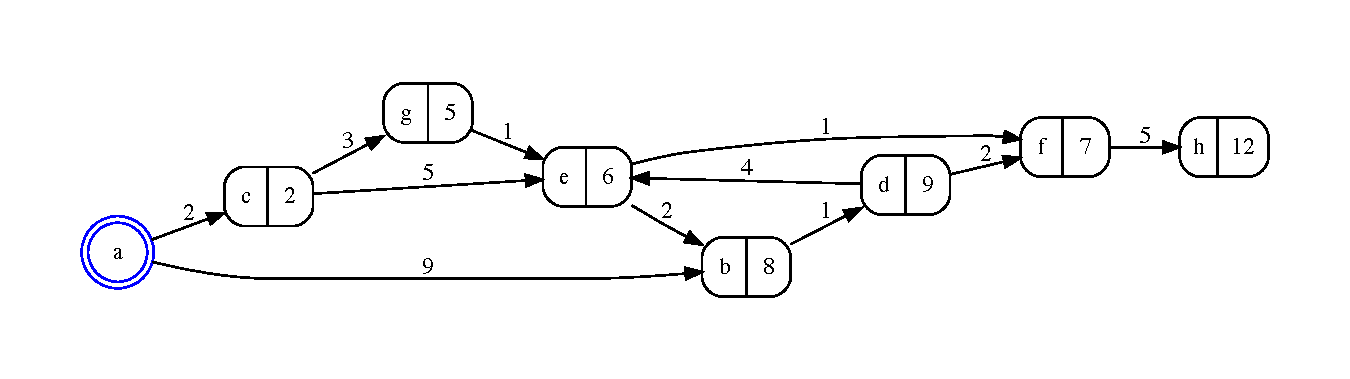
\epsfig{file=Abbildungen/directed-graph.pdf,scale=0.7}
        \caption{A directed graph.}
        \label{fig:directed-graph.pdf}
      \end{figure}
      \end{enumerate}
\item The variable $\mytt{Distance}$ is a \blue{dictionary}.  After the computation is
      finished, for every node $x$ such that $x$ is reachable from the node \mytt{source},
      the value $\mytt{Distance}[x]$ records the length of the shortest path from \mytt{source} to $x$.

      The node $\mytt{source}$ has distance $0$ from the node $\mytt{source}$ and initially this is
      all we know.  Hence, the dictionary $\mytt{Distance}$ is initialized as $\bigl\{\mytt{source}:0 \bigr\}$.
\item The variable $\mytt{Fringe}$ is a list of those nodes that already have an estimate of
      their distance from the  node \mytt{source}.  Furthermore, if a node is in \mytt{Fringe} then this
      node might have neighbouring node whose distance from \mytt{source} hasn't yet been computed. 
      Initially we only know that the node $\mytt{source}$ is connected to the node \mytt{source}.
      Therefore, we initialize the list $\mytt{Fringe}$ as the list
      \\[0.2cm]
      \hspace*{1.3cm}
      $[ \mytt{source} ]$.
\item Every iteration of the \mytt{while}-loop takes the first node \mytt{u} from the \mytt{Fringe}.
\item Next, we compute all nodes $\mytt{v}$ that can be reached from $\mytt{u}$. For every node \mytt{v}
      that can be reached from $\mytt{u}$ by an edge $(u, v)$ we check whether 
      reaching \mytt{v} from \mytt{u} results in a shorter path than previously known.
      There are two cases.
      \begin{enumerate}
      \item If there is an edge from node $\mytt{u}$ to a node $\mytt{v}$ and  $\mytt{Distance}[\mytt{v}]$ is still
            undefined, then we hadn't yet found a path leading to $\mytt{v}$.
      \item Furthermore, there are those nodes $\mytt{v}$ where we had already found a path leading from
            $\mytt{source}$ to $\mytt{v}$ but the length of this path is longer than the length of the path
            that we get when we first visit $\mytt{u}$ and then proceed to $\mytt{v}$ via the edge $(\mytt{u},\mytt{v})$.
      \end{enumerate}
      We compute the distance of the path leading from $\mytt{source}$ to $\mytt{u}$ and then to
      $\mytt{v}$ in both of these cases and add $\mytt{v}$ to the \mytt{Fringe}, provided it isn't
      already a member of the \mytt{Fringe}.
\item The algorithm terminates when the list $\mytt{Fringe}$ is empty because in that case we don't
      have any means left to improve our estimate of the distance function.
\end{enumerate}

\subsection{Dijkstra's Algorithm \label{sec:dijkstra}}
The Bellman-Ford algorithm stores the nodes that are picked next to be examined in the list $\mytt{Fringe}$.
This results in non-optimal behaviour of the algorithm:  A node can be picked from $\mytt{Fringe}$ and
removed from the $\mytt{Fringe}$ only to be reinserted into the $\mytt{Fringe}$ later.  In 1959
\href{https://en.wikipedia.org/wiki/Edsger_W._Dijkstra}{Edsger W.~Dijkstra}\footnote{
  Edsger Wybe Dijkstra received the 1972 Turing Award.}(1930 -- 2002) \cite{dijkstra:59}
published an algorithm that was more careful in picking the nodes from the \mytt{Fringe}.  Dijkstra's algorithm guarantees that it
is never necessary to reinsert a node back into the set $\mytt{Fringe}$.  Dijkstra had the idea to always choose
that node from the \mytt{Fringe} that has the smallest distance to the node $\mytt{source}$.  This has the effect that the algorithm
visits nodes in increasing order of their distance from the node source.  
To implement this, we have to
represent the variable $\mytt{Fringe}$ as a priority queue where the priority of a node $x$ is given by the
distance of $x$ to the node $\mytt{source}$.  Figure \ref{fig:Dijkstra.ipynb} on page
\pageref{fig:Dijkstra.ipynb} shows an implementation of Dijkstra's algorithm 
\index{Dijkstra's algorithm}
in \textsl{Python}.


\begin{figure}[!ht]
\centering
\begin{minted}[ frame         = lines, 
                framesep      = 0.3cm, 
                firstnumber   = 1,
                bgcolor       = sepia,
                numbers       = left,
                numbersep     = -0.2cm,
                xleftmargin   = 0.8cm,
                xrightmargin  = 0.8cm,
              ]{python3}
    def shortest_path(source, Edges):
        Distance = { source: 0 }
        Visited  = { source }
        Fringe   = Set()
        Fringe.insert( (0, source) )
        while not Fringe.isEmpty():
            d, u = Fringe.pop()
            for v, l in Edges[u]:
                dv = Distance.get(v, None)
                if dv == None or d + l < dv:
                    if dv != None:
                        Fringe.delete( (dv, v) )
                    Distance[v] = d + l
                    Fringe.insert( (d + l, v) )
            Visited.add(u)
        return Distance
\end{minted}
\vspace*{-0.3cm}
\caption{Dijkstra's algorithm to solve the shortest path problem.}
\label{fig:Dijkstra.ipynb}
\end{figure}
Since the priority queue that is implemented in \textsl{Python} as the module \mytt{heapq} does not provide a
method to change the priority of an object that is already part of the queue, I have instead used the class
\href{https://github.com/karlstroetmann/Algorithms/blob/master/Python/Set.ipynb}{Set}, which I have implemented
myself.  The notebook \mytt{Set,ipynb} implements sets via \textsc{Avl} trees.  In addition to the methods
\mytt{insert}, \mytt{delete}, and \mytt{isEmpty}, the module \mytt{Set} provides the method
$\mytt{pop}$.  Given a set $S$, the call
\\[0.2cm]
\hspace*{1.3cm}
$S.\mytt{pop}()$
\\[0.2cm]
returns the smallest element from the set $S$.  Furthermore, this element is removed from $S$.
Hence, objects of class \mytt{Set} can be used as priority queues.
We proceed to discuss the program shown in Figure \ref{fig:Dijkstra.ipynb} line by line.
\begin{enumerate}
\item \mytt{Distance} is a dictionary mapping nodes to their estimated distance from the node
      \mytt{source}.  If $d = \mytt{Distance}[x]$, then we know that there is a path of length $d$ leading
      from \mytt{source} to $x$.  However, we do not know whether there is a path shorter
      than $d$ that also connects the source to the node $x$.
\item The program shown in Figure \ref{fig:Dijkstra.ipynb} has an additional variable called $\mytt{Visited}$.
      This variable contains the set of those nodes that have been  \blue{visited} by the algorithm.
      To be more precise, $\mytt{Visited}$ contains those nodes $\mytt{u}$ that have been removed from the
      $\mytt{Fringe}$ and for which all neighbouring nodes, i.e.~those nodes $y$ such that
      there is an edge $(u,y)$, have been examined.  We need the variable \mytt{Visited} in order to prove
      the correctness of the algorithm.  This is explained in more detail later.
\item \mytt{Fringe} is a priority queue that contains pairs of the form $(d, x)$, where $x$ is a node and $d$
      is the distance that $x$ has from the node \mytt{source}.  This priority queue is implemented as a set,
      which in turn is represented by an ordered binary tree.  The fact that we store the node $x$ and the
      distance $d$ as a pair $(d,x)$ implies that the distances are used as priorities because pairs are
      compared lexicographically.
      Initially the only node that is known to be
      reachable from \mytt{source} is the node \mytt{source}.  Hence \mytt{Fringe} is initialized as the
      set $\{ (0, \mytt{source}) \}$.
\item As long as the set \mytt{Fringe} is not empty, line 7 of the implementation removes that node $u$
      from the set \mytt{Fringe} that has the smallest distance $d$ from the node \mytt{source}.
\item Next, all edges leading away from $u$ are visited.  If there is an edge $(u, v)$ that has length $l$,
      then we check whether the node $v$ has already a distance assigned.  If the node $v$ already has the
      distance $\mytt{dv}$ assigned but the value $d + l$ is less than \mytt{dv}, then we have found a
      shorter path from \mytt{source} to $v$.  This path leads from \mytt{source} to $u$ and then proceeds
      to $v$ via the edge $(u,v)$.
\item If \mytt{v} had already been visited before and hence $\mytt{dv}=\mytt{Distance}[v]$ is defined, we
      have to update the priority of the $v$ in the \mytt{Fringe}.  The easiest way to do this is to remove
      the old pair $(\mytt{dv}, v)$ from the \mytt{Fringe} and replace this pair by the new pair
      $(d+l, v)$, because $d+l$ is the new estimate of the distance between \mytt{source} and $v$ and
      $d+l$ is the new priority of $v$.
\item Once we have inspected all neighbours of the node $u$, $u$ is added to the set of those nodes that have
      been \mytt{Visited}.
\item When the \mytt{Fringe} has been exhausted, the dictionary \mytt{Distance} contains the distances of
      every node that is reachable from the node \mytt{source}.  
\end{enumerate}

\begin{Theorem}[Distance Property of Dijkstra's Algorithm]
  If a node $u$ is removed from the \mytt{Fringe} in line 7, then we have
  \\[0.2cm]
  \hspace*{1.3cm}
  $\mytt{sp}(u) = d = \mytt{Distance}[u]$
  \\[0.2cm]
  and every node $w$ such that $\mytt{sp}(w) \leq \mytt{sp}(u)$ satisfies
  \\[0.2cm]
  \hspace*{1.3cm}
  $\mytt{Distance}[w] = \mytt{sp}(w)$.
\end{Theorem}

\proof The claim is proven by induction on $n := \mytt{sp}(u)$.
\begin{description}
\item[Base case:] $n = 0$.

  The only node $u$ satisfying $\mytt{sp}(u) = 0$ is the node $u = \mytt{source}$.
  Initially, the pair $(0, \mytt{source})$ is put onto the \mytt{Fringe} in line 5.
  The only way a pair on the \mytt{Fringe} could be changed is when a pair is removed in line 12 and then
  reinserted in line 14 with a smaller distance.  As there is no smaller distance than $0$, the pair
  $(0, \mytt{source})$ can not be altered.  Therefore, when \mytt{source} is removed from the
  \mytt{Fringe} in line 8, we must have $d = 0$ and hence we have $\mytt{sp}(u) = d$.
  As all of our edges are assumed to be positive natural numbers, there can be no node $w$ such that
  $\mytt{sp}[w] < 0$. Hence the second part of the claim is trivially true in this case.
\item[Induction step:]  We assume that the claim holds for $\mytt{sp}[u] \in \{0,1,\cdots,n-1\}$
  and we prove that this implies that the claim also holds in case that $\mytt{sp}(u) = n$.

  As $\mytt{sp}(u) = n$ there has to be a shortest path
  \\[0.2cm]
  \hspace*{1.3cm}
  $P = [x_0, x_1, \cdots, x_{k-1}, x_k]$
  \\[0.2cm]
  such that $x_0 = \mytt{source}$, $x_k = u$, and $\weight{P} = n$.  Since the lengths of all edges are
  positive natural numbers, this implies that the path $P' = [x_0,x_1, \cdots, x_{k-1}]$ has a length $d'$ such
  that $d' < \mytt{sp}(u) = n$.  By induction hypothesis this implies that
  \\[0.2cm]
  \hspace*{1.3cm}
  $d' = \mytt{Distance}[x_{k-1}] = \mytt{sp}(x_{k-1})$.
  \\[0.2cm]
  Immediately after $\mytt{Distance}[x_{k-1}]$ is computed in line 13, the pair
  $(d', x_{k-1})$ is put on the \mytt{Fringe} in line 14.  Since $d' < d$, this pair is removed from the
  \mytt{Fringe} prior to the pair $(d, u)$.  After the pair $(d',x_{k-1})$ is removed from the
  \mytt{Fringe} in line 7, all edges starting in $x_{k-1}$ are checked in line 8.
  Hence, the edge $(x_{k-1}, x_k)$ has also been checked and, if $\mytt{Distance}[x_k]$ had been greater than
  $d$, it has been reduced to $d$ at that time.  Therefore,
  \\[0.2cm]
  \hspace*{1.3cm}
  $\mytt{Distance}[u] = d = \mytt{sp}(u)$.
  \\[0.2cm]
  A similar argument shows that for all nodes $w$ such that  
  $\mytt{sp}(w) \leq \mytt{sp}(u)$ we must have $\mytt{Distance}[w] = \mytt{sp}(w)$.  \qed
\end{description}

\exercise
Improve the implementation of Dijkstra's algorithm given above so that the algorithm also computes
the shortest path for every node that is reachable from $\mytt{source}$.
\eox


\subsection{Complexity}
If a node $\mytt{u}$ is removed from the priority queue $\mytt{Fringe}$, the node is added to the set
$\mytt{Visited}$.  The invariant that was just proven implies that in that case
\\[0.2cm]
\hspace*{1.3cm}
$\mytt{sp}(u) = \mytt{Distance}[u]$
\\[0.2cm]
holds.  This implies that the node $\mytt{u}$ can never be reinserted into the priority queue
$\mytt{Fringe}$, because a node $\mytt{v}$ is only inserted in $\mytt{Fringe}$ if either 
 $\mytt{Distance}[\mytt{v}]$ is still undefined or if  the  value $\mytt{Distance}[\mytt{v}]$ decreases.  
Inserting a node into a priority queue containing  $n$ elements can be bounded by
$\Oh\bigl(\log_2(n)\bigr)$.  As the priority queue never contains more than $\#\nodes$ nodes,
the first insertion of a node into the priority queue can be bounded by
\\[0.2cm]
\hspace*{1.3cm}
$\Oh\bigl(\#V \cdot \log_2(\#V)\bigr)$.
\\[0.2cm]
We also have to analyse the complexity of removing a node from the fringe and then reinserting this node.
The number of times the assignment
\\[0.2cm]
\hspace*{1.3cm}
\mytt{Fringe -= \{ [dvOld, v] \};} 
\\[0.2cm]
is executed is bounded by the number of edges leading to the node $\mytt{v}$.
Removing an element from a set containing $n$ elements can be bounded by
 $\Oh\bigl(\log_2(n)\bigr)$.  Hence, removal of all nodes from the Fringe can be bounded by
\\[0.2cm]
\hspace*{1.3cm}
$\Oh\bigl(\#\edges \cdot \log_2(\#\nodes)\bigr)$.
\\[0.2cm]
Here,  $\#\edges$ is the number of edges.  Hence the complexity of Dijkstra's algorithm can be
bounded by the expression \\[0.2cm]
\hspace*{1.3cm} $\Oh\bigl((\#\edges + \#\nodes) * \ln(\#\nodes)\bigr)$. \\[0.2cm]
If the number of edges leading  to a given node is bounded by a fixed number, e.g.~if there
are at most 4 edges leading to a given node, then the number of edges is a fixed multiple of the
number of nodes.  In this case, the complexity of 
 Dijkstra's algorithm is given by the expression  
\\[0.2cm]
\hspace*{1.3cm}
$\Oh\bigl(\#\nodes * \log_2(\#\nodes)\bigr)$.

\section{Topological Sorting}
\index{topological sorting}
Assume that you have a huge project to manage.  In order to do so, you can use 
\href{https://en.wikipedia.org/wiki/Program_evaluation_and_review_technique}{\textsc{Pert}}, which is short for
\blue{\underline{p}rogram \underline{e}valuation and \underline{r}eview \underline{t}echnique}.  Using \mytt{Pert},
you break your project into a number of \blue{tasks}
\\[0.2cm]
\hspace*{1.3cm}
$T := \{t_1,\cdots,t_n\}$.  
\\[0.2cm]
Furthermore, there are \blue{dependencies} between the task: These dependencies take the form $s \prec t$, where $s$ and
$t$ are tasks.  A dependency of the form $s \prec t$ means that the task $s$ has to be finished before the task $t$
can start.  For example, if the overall project is to get dressed in the morning\footnote{
  In order to keep things manageable, I have made the assumption that the person that needs to get dressed is male.
}, the set $T$ of task is given
as follows:
\\[0.2cm]
\hspace*{1.3cm}
$T := \{ \textsl{socks}, \textsl{trousers}, \textsl{shirt}, \textsl{shoes} \}$.
\\[0.2cm]
The elements of $T$ are interpreted as follows:
\begin{itemize}
\item \textsl{socks}: Put on socks.
\item \textsl{trousers}: Put on trousers.
\item \textsl{shirt}: Put on shirt.
\item \textsl{shoes}: Put on shoes.
\end{itemize}
There are some \blue{dependencies} between these tasks:  For example, putting on the shoes first and then trying to
put on the socks does not work well.  In detail, we have the following dependencies between the different tasks:
\begin{enumerate}
\item $\textsl{socks} \prec \textsl{shoes}$,
\item $\textsl{trousers} \prec \textsl{shoes}$,
\item $\textsl{shirt} \prec \textsl{trousers}$.
\end{enumerate}
Now the problem is to order the tasks such that the dependencies are satisfied.  For example, for the project
of dressing up in the morning, the following schedule would work:
\\[0.2cm]
\hspace*{1.3cm}
\textsl{socks}, \textsl{shirt}, \textsl{trousers}, \textsl{shoes}.
\\[0.2cm]
Of course, the project of dressing up is trivial.
However, complex projects can have ten thousands of tasks and even more dependencies between these tasks.  For
example, the US-lead invasion in the second Irak war was a project consisting of more than $30\,000$ tasks.
It is rumoured that the plan for the US invasion of the
\href{https://en.wikipedia.org/wiki/China}{People's Republic of China}  
contains an excess of 2 million tasks!  Ordering the tasks for a project of this size is very difficult to do by
hand.  Instead, a technique called \blue{topological sorting} is used. 

In computer science, the utility program \href{https://edoras.sdsu.edu/doc/make.html}{\mytt{make}} uses
topological sorting to execute the commands necessary to build a software system in the right order.

\subsection{Formal Definition of Topological Sorting}
In order to better grasp the idea of a topological sorting problem, we define it formally as a graph
theoretical problem.
\begin{Definition}[Topological Sorting Problem, Solution of a Topological Sorting Problem]  \hspace*{\fill} \\
  \index{topological sorting problem}
  A \href{https://en.wikipedia.org/wiki/Topological_sorting}{topological sorting problem} is a finite directed graph
  $\pair(T, D)$ where
  \begin{itemize}
  \item $T$ is a finte set that is called the set of \blue{tasks} and 
  \item $D \subseteq T \times T$ is called the set of \blue{dependencies}.

        If $\pair(s, t) \in D$, then this is written as 
        \\[0.2cm]
        \hspace*{1.3cm}
        $s \prec t$, \quad which is read as $t$ \blue{depends} on $s$.
  \end{itemize}
  For conciseness, we abbreviate ``topological sorting problem'' as \textsc{Tsp}.
  A \blue{solution} of a topological sorting problem is a list $S$ such that
  \begin{enumerate}[(a)]
  \item every task $t \in T$ appears exactly once in $S$, i.e.~we have
        \\[0.2cm]
        \hspace*{1.3cm}
        $\forall t \in T: \exists k \in \mathbb{N}: S[k] = t$.
\item If there are two tasks $t_1, t_2 \in T$ such that $t_1 \prec t_2$, then $t_1$ appears before $t_2$
        in the list $S$, i.e.~we have
        \\[0.2cm]
        \hspace*{1.3cm}
        $\forall i,j \in \bigl\{1,\cdots,\mytt{len}(S)\bigr\}:\bigl(S[i] \prec S[j] \rightarrow i < j\bigr)$.
        \eox
\end{enumerate}

\end{Definition}

\subsection{Computing the Solution of a \textsc{Tsp}}
Next, we present \href{https://en.wikipedia.org/wiki/Topological_sorting}{Kahn's algorithm}\index{Kahn's algorithm} \cite{kahn:1962} for solving a \textsc{Tsp}.
The basic idea is very simple. Ask yourself:  How can a list $S$ that is supposed to be a solution to a
\textsl{Tsp} $\pair(T, D)$ start? 
Of course, it can only start with a task that does not depend on any other task.  Therefore, if we are
unfortunate and every task depends on some other task, there is no way to solve the \textsc{Tsp}.  Otherwise,
we can just pick any task that does not depend on another task to be the first task and remove it from the set
of tasks.  After that it's just rinse and repeat.  Therefore, Kahn's algorithm for solving a \textsc{Tsp}
$\pair(T, D)$ works as follows: 
\begin{enumerate}
\item Initialize the list $\mytt{S}$ of tasks to the empty list.
\item Pick a task $t \in T$ that does not depend on any other task and append this task to $\mytt{S}$.

      If there is no such task, the \textsc{Tsp} is not solvable and the algorithm terminates with failure.
\item Remove the task $t$ from both $T$ and $D$, i.e.~if there is a pair $\pair(t, s) \in T$ for some $s$, then
      this pair is removed from $D$.
\item If $T$ is not yet empty, go back to step 1.  
\end{enumerate}
When the algorithm terminates, the list \mytt{S} is a solution to the \textsc{Tsp} $\pair(T, D)$.

In order to implement this algorithm we need to think about the data structures that are needed.
In order to be able to pick a task $t \in T$ that does not depend on any other task, we need a set of all those
tasks that do not depend on any other task.  Using a graph theoretical manner of speaking we call this set the
set of \blue{orphans}, since in graph theory, if we have an edge $\pair(s, t)$, then $s$ is called a parent of
$t$ and, therefore, a node with no parents is called an \blue{orphan}.  In order to maintain the set of
orphans, we need to be able to compute the \blue{parents} of each node.  Furthermore, when we remove a node $t$
from the graph after inserting it into the list \mytt{S}, we have to compute the set of children of that
node.  The reason is that we have to update the set of parents of the children of $t$.  This leads to the algorithm
shown in Figure \ref{fig:Topologocal-Sorting.ipynb} on page \pageref{fig:Topologocal-Sorting.ipynb}.

\begin{figure}[!ht]
\centering
\begin{minted}[ frame         = lines, 
                framesep      = 0.3cm, 
                firstnumber   = 1,
                bgcolor       = sepia,
                numbers       = left,
                numbersep     = -0.2cm,
                xleftmargin   = 0.0cm,
                xrightmargin  = 0.0cm,
              ]{python3}
    def topo_sort(T, D):
        Parents  = { t: set() for t in T }  # dictionary of parents
        Children = { t: set() for t in T }  # dictionary of children
        for s, t in D:
            Children[s].add(t)
            Parents [t].add(s)
        Orphans = { t for t, P in Parents.items() if len(P) == 0 }
        Sorted  = []
        while len(T) > 0:
            assert Orphans != set(), 'The graph is cyclic!'
            t        = arb(Orphans)
            Orphans -= { t }
            T       -= { t }
            Sorted.append(t)
            for s in Children[t]:
                Parents[s] -= { t }
                if Parents[s] == set():
                    Orphans.add(s)
        return Sorted
\end{minted}
\vspace*{-0.3cm}
\caption{Kahn's algorithm for topological sorting.}
\label{fig:Topologocal-Sorting.ipynb}
\end{figure}

\begin{enumerate}
\item In order to compute the parents and children of a given node efficiently, Kahn's algorithm
      uses two dictionaries: $\mytt{Parents}$ and $\mytt{Children}$.
      In lines 2 and 3 we initialize these dictionaries to be empty and the \mytt{for}-loop in line 4 fills both of these
      dictionaries: If there is a dependency $\pair(\mytt{s}, \mytt{t})$, then $\mytt{t}$ is a child of
      $\mytt{s}$ and $\mytt{s}$ is a parent of $\mytt{t}$.  Therefore, $\mytt{t}$ is added to the set
      $\mytt{Children[s]}$ and $\mytt{s}$ is added to the set $\mytt{Parents[t]}$.
\item In line 7, we compute the set $\mytt{Orphans}$.  This is the set of those tasks that have no
      $\mytt{Parents}$.  We can start with any task from this set.
\item In line 8, the list $\mytt{Sorted}$ is initialized.  When the algorithm completes without failure, this list will
      contain a solution of the \textsc{Tsp}.
\item As long as there are still tasks in the set $\mytt{T}$ that have not been inserted into the list
      $\mytt{Sorted}$ the algorithm keeps going.
\item If at any point the set of tasks $\mytt{T}$ that need to be scheduled is not yet empty but all remaining
      tasks still have parents, i.e.~they depend on the completion of some other task, then the given \textsc{Tsp}
      is cyclic and hence not solvable and therefore the algorithm terminates with a failure message.
\item Otherwise, we remove a task $\mytt{t}$ from the set of orphaned tasks, remove this task from $\mytt{T}$
      and append it to the list of scheduled tasks $\mytt{Sorted}$.
\item Finally, we have to update the parent dictionary so that for all children $\mytt{s}$ of the task
      $\mytt{t}$, the task $\mytt{t}$ is no longer a parent of the task $\mytt{s}$.  Furthermore, if this
      implies that the task $\mytt{s}$ has no parents left, it needs to be added to the set $\mytt{Orphans}$.
\end{enumerate}

\subsection{Complexity}
If the number of dependencies that any given task is involved in is bounded by some fixed constant and $n$ is
the number of tasks,  then the complexity of Kahn's algorithm as given in Figure \ref{fig:Topologocal-Sorting.ipynb}
is  
\\[0.2cm]
\hspace*{1.3cm}
$\Oh\bigl(n \cdot \log_2(n)\bigr)$.
\\[0.2cm]
The reason is that building the dictionary \mytt{Parents} as well as the dictionary \mytt{Children} both
have the complexity $\Oh\bigl(n \cdot \log_2(n)\bigr)$. Furthermore, maintaining  the set \mytt{Orphans} also
has a complexity of
$\Oh\bigl(n \cdot \log_2(n)\bigr)$.

%%% Local Variables: 
%%% mode: latex
%%% TeX-master: "algorithms"
%%% End: 
